This chapter will take a more in-depth look at CI/CD. Some of the core terms, concepts and technologies commonly used in CI/CD practices will be described and explained. An overview of Certidude will be given as well.

\section{Certidude}
Certidude is an open-source CA management tool mainly designed for VPN gateway operators to make VPN client setups on laptops, desktops and other devices easier.\cite{certidude} Certidude allows for easy signing, revoking and review of (authorized) X.509 certificates and CSRs (Certificate Signing Request) used in establishing VPN tunnels and accessing a company's PKI (Public Key Infrastructure) as a whole. It integrates with authentication protocols like LDAP (Lightweight Directory Access Protocol) and Kerberos and is able to provide CRLs (Certificate Revocation Lists) and OCSP (Online Certificate Status Protocol) responses to querying gateways ensuring the validity of presented certificates. See Figure \ref{fig:certidude} for an overview of Certidude and how it relates to other services.

\begin{figure}[ht]
    \centering
    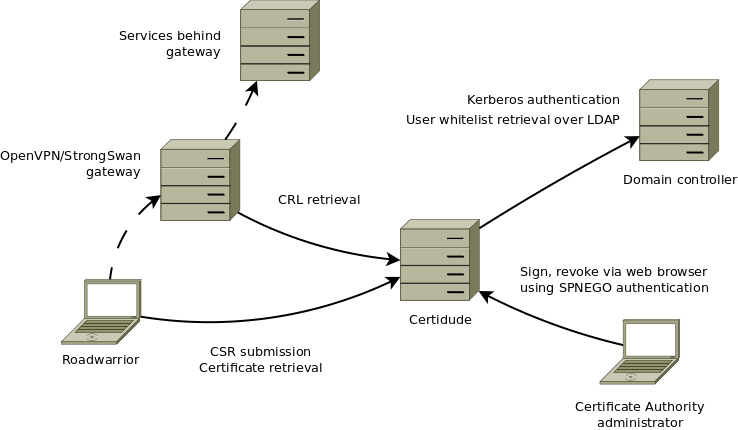
\includegraphics[width=\textwidth]{figures/certidude2.png}
    \caption{\textit{An overview of Certidude and integrated services.}\cite{certidude}}
    \label{fig:certidude}
\end{figure}

\section{Continuous Integration, Delivery, Deployment}\label{sec:continuous-practices}
Continuous practices revolve around using adequate version control systems, integrating code often and fixing code the moment it becomes apparent it has broken. It plays well with other development practices like TDD (Test Driven Development) and refactoring because of their focus on incremental changes and improvements.\cite{ci-duvall} Adhering to these types of best practices allow for companies to frequently and reliably release new features and products, consequently adding business value.\cite{cicd-review}

The generic set of Continuous practices can be subdivided in logical parts. Defining where practicing Continuous Integration, Delivery or Deployment start and stop seems however to be a somewhat hard task to execute since no official consensus exists. The definition for Continuous Integration that seems by far most popular is that of Martin Fowler from his popular "\textit{Continuous Integration}" article:

\textit{"Continuous Integration is a software development practice where members of a team integrate their work frequently, usually each person integrates at least daily - leading to multiple integrations per day. Each integration is verified by an automated build (including test) to detect integration errors as quickly as possible."}\cite{ci-duvall,cicd-review,fowler,cd-casestudy,devops-implementation}

Continuous Delivery generally aims to ensure that an application under development is production-ready at all times and combines Continuous Integration with the \textit{possibility} of deployment automation.\cite{cicd-review,deploymentvdelivery,continuous-delivery} This means that at any time, code present in the shared repository should be deployable and should have passed all tests. Benefits for associated practices have been a reduced deployment risk (less can go wrong with small changes) and more immediate user feedback (develop only useful software).\cite{cicd-review,continuous-delivery}

Continuous Deployment adds to Continuous Delivery by actually automatically deploying code to a production server the moment tests are passed. It's goals seem to overlap with those of Continuous Delivery. The main difference is its push-based approach, as opposed to Continuous Delivery's pull based approach where a later review process determines what actually gets deployed.\cite{cicd-review,deploymentvdelivery,continuous-deployment}

\pagebreak

A lot of tasks and best practices associated with CI/CD allow for them to be automated: automatic unit/integration testing, automatic code quality scans, automatic deployment of code, automatic packaging and automatic reporting on all of the above. Various automated build servers have emerged to make the life of developers and administrators easier and which often allow for many native and 3rd party tool integrations.

The purpose of these integrations and tools are varied. The following use cases are merely a subset:\cite{cicd-review} 
\begin{itemize}
    \item Reduce test and build time 
    \item Increase visibility and awareness on build and test results
    \item Detect violations, flaws and faults
    \item Address security and scalability issues
\end{itemize}

Defining the steps and components these build servers need come with their own associated jargon.\cite{oss-tdd} A high level overview can be seen in Figure \ref{fig:pipeline-overview} which consists of the following building blocks:
\begin{itemize}
    \item \textbf{Job} or \textbf{Task}: a series of sequential instructions (e.g. code checkout through git)
    \item \textbf{Stage}: a collection of jobs that could be executed non-sequentially (e.g. test phase)
    \item \textbf{Pipeline}: a collection of stages that are executed sequentially
\end{itemize}

\begin{figure}[ht]
    \centering
    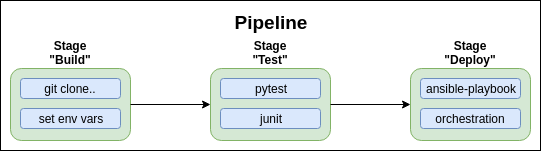
\includegraphics[width=\textwidth]{figures/drawio/pipeline_overview.png}
    \caption{\textit{An overview of CI/CD building blocks}}
    \label{fig:pipeline-overview}
\end{figure}

\pagebreak

Historically these different jobs, stages and pipelines were commonly configured through GUI-based web form submissions and other abstractions which distanced programmers from their build configurations.\cite{intro-pipeline-as-code,jenkins-pipeline} This approach had other problems like being unable to track changes to build configurations, which result in non-reproducible builds and the inability for programmers to change the pipeline that resides on a centralized build server.\cite{what-pipeline-as-code}


The build-as-code approach introduced by TravisCI popularized the idea that the pipeline configuration is part of the same VCS (Version Control System) repository as the software project it is supposed to build and test. On top of that its pipeline configuration was done in a human-readable format through a declarative syntax using YAML files.\cite{what-pipeline-as-code}

Next generation CI/CD build servers introduced the capability to configure pipelines through full programming languages or specialized DSLs (Domain Specific Language) which also became part of the VCS repository. This added complexity to the writing of pipelines but allowed for the setup of more complex pipelines through the use of parameterization, conditional execution and other language constructs as well.\cite{what-pipeline-as-code} Some other advantages could be syntax-highlighting and auto-complete in modern IDEs (Integrated Development Environments). Some examples include:
\begin{itemize}
    \item TeamCity's Kotlin-based DSL as an alternative to their XML format.\cite{teamcity-dsl}
    \item Jenkins's Groovy-based DSL.\cite{jenkins-dsl}
    \item Gomatic through Python.\cite{gomatic-gpl}
\end{itemize}

Currently it is common for declarative pipeline definition syntaxes to include functionality like conditional execution and inheritance as well. These include TravisCI, GitlabCI (both use YAML files) and the previously mentioned Jenkins that also supports a declarative pipeline definition syntax.\cite{jenkins-declarative}

\pagebreak

\section{Pipeline Integrations}
This section will shortly discuss some of the type of tools that are commonly used in CI/CD pipelines. This should help to illustrate the power and flexibility of CI/CD servers, their applicability in the field of Cyber-Security as well as prepare for Chapter \ref{chapter:analysis} and Chapter \ref{chapter:implementation}, where some of these are implemented and/or compared.

Once a CI/CD automation server is present, it opens up the door to define a large amount of pipelines, stages and jobs that utilize a wide variety of native and third-party tools. Figure \ref{fig:deployment-pipeline} shows some of these, including CI servers themselves. Some of these are generic and usable for all programming languages, others are language specific or assume a specific type of application under development. Since Certidude is a Python based application the focus is on those tools that provide support for it, but most if not all type of tools have Python specific analogous implementations or are language independent.

\begin{figure}[ht]
    \centering
    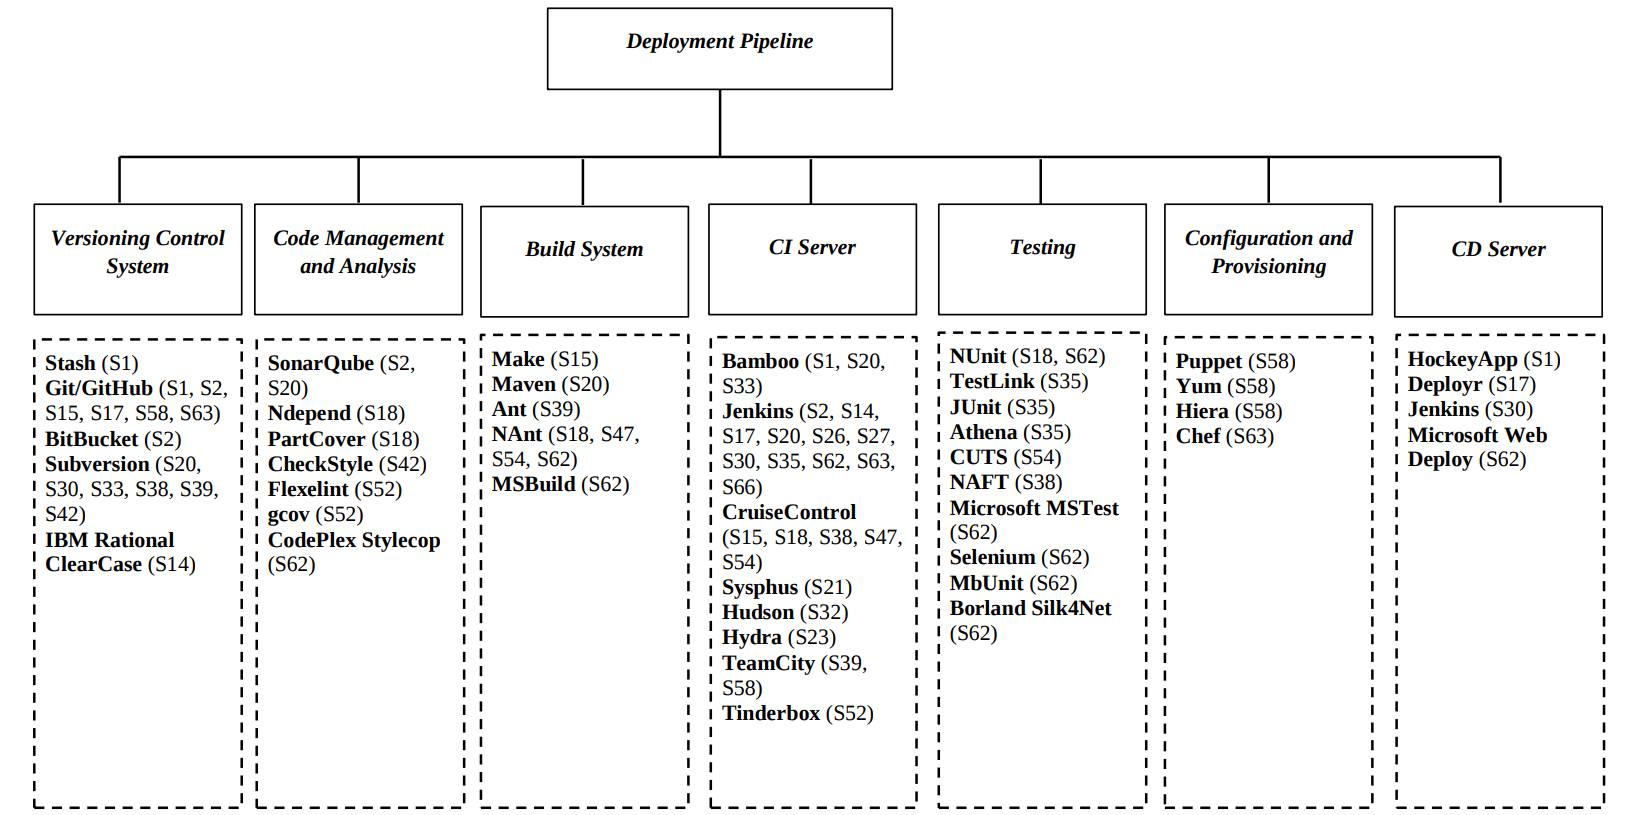
\includegraphics[width=\textwidth]{figures/deployment_pipeline.png}
    \caption{\textit{An overview of tools used in CI/CD pipelines.}\cite{cicd-review}}
    \label{fig:deployment-pipeline}
\end{figure}

\subsection{Build Agent}
As could be seen in Figure \ref{fig:pipeline-overview}, we need to execute some commands and run utilities during our build, test and deploy stages in the pipeline. The question then arises: where are these executed? Some CI/CD servers allow for build agents to be installed on machines which will either listen for incoming requests or fetch user-defined instructions for execution through an API (Application Programming Interface). These can be UNIX machines executing bash scripts but also Windows devices executing PowerShell commands.\cite{gitlab-shell} They capture output of these instructions and feed this and more back to the main CI/CD server. See Figure \ref{fig:cicdserver-agent} for a high-level overview.

\begin{figure}[ht]
    \centering
    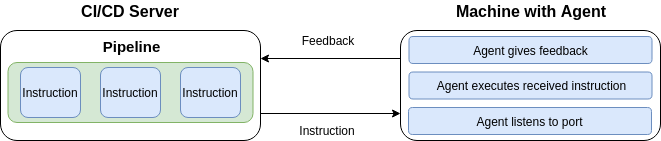
\includegraphics[width=\textwidth]{figures/drawio/cicdserver-agent.png}
    \caption{\textit{High-Level view of a CI/CD server agent interaction}}
    \label{fig:cicdserver-agent}
\end{figure}

While agents can often be installed on any host machine, they are commonly set-up in or setup to control virtualized environments like virtual-machines or containers. This ensures a clean build environment each time the agents receives and runs pipeline instructions. This is important because this allows for dependencies to be more accurately identified, software is tested in the same environment each time tests are run and the test environment can be \textit{exactly} the same as production.

The exact inner workings of virtualization technology is out of scope for this thesis, however it is important to talk about some of their fundamentals, popular implementations and differences.

\subsubsection{VMs} \label{subsec:VMs}
Virtual Machines are emulations of computer systems which provide the same functionality as physical computers. They are generally referred to as \textit{"guests"} while the computing environment within which they are run are referred to as \textit{"hosts"}. Microsoft's documentation describes running a virtual machine as: \textit{"...creating a computer within a computer."}\cite{azure-vm} 

On a typical system the OS's kernel, or supervisor, is the piece of software that is interacting closest with the underlying hardware.
To get things done applications make system calls to the kernel which has higher privileges and in turn grants access to physical resources like memory and the CPU (Central Processing Unit). The kernel of a VM (Virtual Machine) however is presented with virtual resources and its access to hardware is validated and controlled by the host machine. This isolates the host from one, or potentially many VMs running on top of it. To have virtualization capabilities requires what's called a \textit{hypervisor}, also called the supervisor of the supervisor.\cite{virt-dummy,what-is-hypervisor} 

\pagebreak

In practice this can be implemented in software as well as be enabled through special flags in a CPU's architecture instruction set.\cite{virtualbox-virt,hardware-virt} This mechanism of having different levels of privilege is also referred to as ring-protection and is meant to make it harder for common applications, or VMs in this case, to maliciously and/or accidentally crash or corrupt the whole system they are running on.\cite{computerphile-virt}  See Figure \ref{fig:protection-rings} for an overview of protection rings where a hypervisor would run in ring -1.

Virtual Machines are also important because they allow for snapshots, capturing the exact state of a system at a specific point in time and allow for rollback to that state. After a snapshot is made each change to the system is recorded. Rolling back means throwing away those changes.\cite{virtualbox-snap} This enables CI/CD agents to be installed on clean VMs, a snapshot to be created, let these agents execute steps in the build process like installing dependencies, running the code under test, run the tests on that code then report back to the CI/CD server and restore the original state. This level of insight into and control over machine state and code dependencies increases confidence that the code under test will run on production machines as expected.

\begin{figure}[ht]
    \centering
    \includegraphics[width=.5\textwidth]{figures/privilege_rings.png}
    \caption{\textit{Overview of protection rings.}\cite{protection-rings}}
    \label{fig:protection-rings}
\end{figure}

% TODO: Still mention type 1 paravirtualization / type 2 hw-accellerated virtualization through CPU flags / CPU opcodes vm-enter vm-exit..
%       LXD would be a "type 3" linux-only hypervisor.

\subsubsection{Containers}  \label{subsec:containers}
OS-level virtualization, or in its common name "\textit{container}"-technology, is different from traditional VMs and is sometimes described as somewhere between a chroot and a full-blown VM.\cite{lxc} Chroot-environments are a way to isolate processes and applications in a sub-tree of the file system and resembles \textit{installing an OS into your existing OS}.\cite{basic-chroot} This means that one or multiple containers running on a host all share the same kernel with the host instead of having their own. Some popular implementations are BSD-jails\cite{bsd-jail}, LXC\cite{arch-lxc} (Linux Container) and Docker\cite{arch-docker}. Linux based containers (e.g. Docker and LXC) build on top of chroot-environments by using cgroups for resource management \cite{arch-cgroups}, AppArmor / SELinux profiles for security \cite{lxc-intro} and namespaces for isolation.\cite{docker-namespace,evans-container}

\pagebreak

They provide similar capabilities as full-virtualization but with less overhead, making them faster. There are daemons available to help build and manage container instances and their resources (e.g. amount of memory) like iocage\cite{iocage-zfs}, the Docker daemon\cite{arch-docker} and LXD\cite{dustin-lxc} (Linux Container Daemon). These can also be setup to run on modern file systems like ZFS adding services like integrity checking, compression and COW (Copy On Write) snapshotting.\cite{dustin-lxc} Container platforms and orchestration/management tools like OpenShift, Docker Swarm, Docker Compose and Kubernetes are also often used in CI/CD pipelines, especially in large infrastructures, but are out of scope for this work.\cite{openshift,docker-swarm,kubernetes}

\subsubsection{Security Implications for Virtualization Technologies}
Since containers share resources between each other and the host, there have been various high-severity vulnerabilities that can affect services, users and data that make use of them. Some of these also affect VMs and are:
\begin{itemize}
    \item \textbf{Meltdown / Spectre}. These are vulnerabilities that exploit race conditions in privilege checking vs. actual memory access and an optimization technique called branch-prediction to extract data from CPU cache and memory.\cite{meltdown,spectre} 
    \item \textbf{DirtyCow}. Exploits a file/memory access race condition in the Linux kernel which allows an unprivileged user to gain write access to files it shouldn't be able to and become root.\cite{dirty-cow} The name stems from the copy-on-write mechanism that allows for resource sharing as long as it remains unchanged. If it is, a copy is made which is altered and the resource is no longer shared. This exploit allows for changing the original version of those resources.
\end{itemize}
Most CI/CD cloud providers make heavy use of virtualized infrastructure that is shared between all hosted projects. One should be aware that such exploits exist when using cloud-based agents or cloud-based deployments in general.

%DAC by extending non-root "nobody" users that run the container into the host filesystem. So if escape from container possible only rw access to that user's files which shouldnt have a lot.. % this comes from the LXD presentation..

\subsubsection{CWRAP}
CWRAP is a set of tools which are able to create things like privilege separation and isolated network environments.\cite{cwrap} This allows one to test complex server-client interactions on a single host, something Certidude's test suite has. It is an alternative to full-blown VMs or Linux namespaces which are used in container technology (See also section \ref{subsec:VMs} and \ref{subsec:containers}) and is used by projects like Samba to run their test suite with. It comes with less overhead and support on BSDs (as opposed to Docker / LXC which make use of Linux kernel-specific capabilities) but also increased complexity.\cite{cwrap2, cwrap3, cwrap4}

\pagebreak

\subsubsection{Build agent overview}
Figure \ref{fig:build-agents} illustrates the high-level architecture of a host system, the CI/CD build agent and virtualization technologies in which code can be built, run and tested.

% Make this draw.io pictures showing differences VM and containers and our agent running in userland..
%Insert image displaying VM vs Container / CICD agent
\begin{figure}[H]
    \centering
    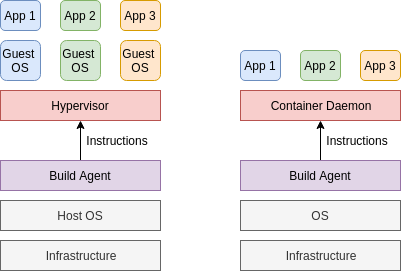
\includegraphics[width=.7\textwidth]{figures/drawio/build-agent.png}
    \caption{\textit{Overview of build agents and their relation to virtual infrastructure.}}
    \label{fig:build-agents} 
\end{figure} 


\subsection{Security Tools} \label{subsec:security}
There are many automated security tools available that can analyze static code or programs during execution to find known vulnerabilities or point to functions/behavior that could be indicative of an underlying problem. Some DAST-tools (Dynamic Application Security Testing) are specialized in exposing web application related vulnerabilities by fuzzing APIs or performing automated SQL (Structured Query Language) injection attacks while SAST-tools (Static Application Security Testing) might look at insecure configuration options or imports of vulnerable libraries.\cite{owasp-tools,owasp-sast} Some CI/CD solutions offer "\textit{Security as a Service}"-support and use similar SAST/DAST tools under the hood.\cite{gitlab-sast,gitlab-dast} There are tools available that manage and analyze code dependencies and any binaries or other artifacts that might get produced as well.\cite{jfrog}

The following list of tools is by no means comprehensive, but are merely some that are either widely used, open-source or have good Python integrations. Some of these will also be discussed during the implementation phase described in Chapter \ref{chapter:implementation}.

\pagebreak

\subsubsection{Clair}
Clair is a container analysis tool that looks for known vulnerabilities in dependencies and libraries used in container recipes.\cite{clair,clair-scanner} It looks at the various layers that comprise a container and checks against multiple open databases and bug trackers to see if one of these is included in the container. Some of these databases include NIST NVD (National Vulnerability Database), Alpine SecDB, RedHat Security Data and Ubuntu CVE tracker (Common Vulnerabilities and Exposures).\cite{clair}

\subsubsection{Bandit}
Bandit is a linter, SAST and code analysis tool that finds common security issues in Python code.\cite{bandit} It supports generating reports in JSON (JavaScript Object Notation), HTML (Hypertext Markup Language) and XML among others. Its modules look for weak ciphers used, hardcoded passwords, insecure deserialization using \textit{pickle} and usage of the \textit{eval} command to just name a few. Although one can also write their own modules for it. Analyzing your code can be done fairly easily through issuing a simple command like in Figure \ref{fig:bandit-command}.

\begin{figure}[H]
\centering
\begin{lstlisting}[frame=single, basicstyle=\small, linewidth=\textwidth]
bandit -r path/to/your/python/code -f xml -o bandit-results.xml 
\end{lstlisting}
\caption{\textit{Example Bandit analysis command.}}
\label{fig:bandit-command}
\end{figure}
Many CI/CD servers allow for some sort of artifact uploading, either natively or through the use of plugins. If there is support for the specific format of the test results these can sometimes be nicely parsed and visualized in the CI/CD server, but reports can alternatively be uploaded to the server's artifact repository for later manual analysis. Figure \ref{fig:bandit-output} is part of the \textit{Bandit} report that was created when the previous command was run on the example application that was developed during the analysis phase described in Chapter \ref{chapter:analysis}.

\begin{figure}[H]
\centering
\begin{lstlisting}[frame=single, basicstyle=\small, linewidth=\textwidth]
Test results:b201_flask_debug_true.html
>> Issue: [B201:flask_debug_true] A Flask app appears to be run 
          with debug=True, which exposes the Werkzeug debugger 
          and allows the execution of arbitrary code.
   Severity: High   Confidence: Medium
   Location: example/app.py:55
   More Info: https://bandit.readthedocs.io/en/latest/plugins/
              b201_flask_debug_true.html
54	if __name__ == '__main__':
55	    app.run(host='0.0.0.0', port=80, debug=True)
\end{lstlisting}
\caption{\textit{Bandit analysis result output.}}
\label{fig:bandit-output}
\end{figure}

\subsubsection{SonarQube}
SonarQube can find code smells, bugs and security vulnerabilities in code.\cite{sonarqube} It provides a CLI (Command Line Interface) scanning tool and databases with known vulnerabilities to do so. It can also nicely visualize \textit{Pytest}, \textit{Coverage}, \textit{Pylint} and \textit{bandit} reports if they are formatted in either JUnitXML or JSON notation. Some of these and their alternatives will also be discussed in section \ref{subsec:other}. It is an interesting tool to help combat regression and security issues by generating, combining and visualizing code quality metrics. 


\subsubsection{Black Duck}
Black Duck is a security tool that can perform binary analysis (e.g. executables and archives), dependency analysis and file system scans to detect vulnerabilities. It integrates with large deployment frameworks like RedHat OpenShift to perform automated scans on container clusters. It can also identify potential license conflicts that arise due to imported code.\cite{black-duck}

\subsubsection{OpenSCAP}
SCAP (Security Content Automation Protocol) is a framework of open standards maintained by NIST and OpenSCAP is a set of tools used to implement this standard which allows for automated configuration and vulnerability scans of computer systems.\cite{mitre-oval} It can do this through the use of XCCDF (Extensible Configuration Checklist Description Format) and OVAL (Open Vulnerability and Assessment Language) files which consist of XML-based descriptions of machine state and system information and link these to security issues.\cite{openscap,openscap-manual} When for example a new vulnerability is discovered, one can write such a file describing the conditions in which the vulnerability appears. Tools like the by OpenSCAP provided \textit{oscap,} are able to scan through these files and discover if any of these described conditions occur on the system it is running on. Repositories for these files are published by companies and projects like Cisco, RedHat, Debian and NIST (National Institute of Standards and Technology).\cite{oval-repo} There are also enterprise level integrations in the form of RedHat container vulnerability management (Atomic Scan) and system management through RedHat Satellite profiles.\cite{openscap-tools}

\pagebreak

\subsubsection{OWASP ZAP}
The ZAP project is an open-source security testing tool supported by OWASP (Open Web Application Security Project). It can be set-up in between a browser and a web application as a proxy and analyzes traffic during interactions to detect common vulnerabilities like SQL-injections. It supports both passive scans as well as active scans of your web application using a wide variety of extensions.\cite{owasp-zap,owasp-zap-ext} See also section \ref{subsec:other} for information on Selenium Web browser, in combination of which this could be used to automate security tests.

\subsection{Other} \label{subsec:other}
\subsubsection{Functional Testing}
A framework that is often used for automated functional testing of web applications and their GUIs is \textit{Selenium WebDriver} which can run tests against many popular browsers like Chrome, Firefox, Edge and Safari.\cite{selenium} It does this by obfuscating away any actual HTML interactions from the tests through what's called a PageObject pattern.\cite{fowler-page} It has good integrations with Python as well.\cite{selenium-python}

\subsubsection{Code Coverage}
Writing and passing tests should raise the confidence one has in the proper functionality of the code under test. But how does one know how well these tests reflect the code's functionality? Code coverage refers to metrics that reflect how much code has been executed during the running of tests. They can be a measure of how well tests are written since a higher coverage percentage reduces the chance of any bugs remaining in the code. They generally come in a few forms: \textit{branch coverage}, \textit{statement coverage}, \textit{function coverage} and \textit{condition coverage}. High code coverage percentages don't guarantee high quality of code.\cite{cov-misuse} And 100\% statement coverage does not guarantee 100\% branch coverage, as can be seen in the example in Figure \ref{fig:codecoverage} where, given test situation \textit{a='true'} and \textit{b='true'}, there is 100\% statement coverage but two-thirds of the branches are not covered.

\begin{figure}[!htb]
    %\begin{minipage}{0.5\textwidth}
    \begin{subfigure}[b]{0.5\textwidth}
    \begin{lstlisting}[frame=single, basicstyle=\small, linewidth=.9\textwidth]
# given a=true and b=true
if(a){
    if(b){
        bool example = true;
    }
}
    \end{lstlisting}
    \end{subfigure}
    %\end{minipage}%
    %\begin{minipage}{0.5\textwidth}
    \begin{subfigure}[b]{0.5\textwidth}
    \centering
    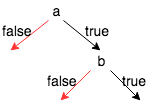
\includegraphics[width=.75\textwidth]{figures/branch-statement.png}
    \end{subfigure}
    %\end{minipage}
    \caption{\vspace{-3mm}\textit{Branch coverage vs. Statement coverage.}\cite{stack-cov}}
    \label{fig:codecoverage}
\end{figure} 

There are tools that can create these reports for most popular languages and Python is no exception to this. \textit{Coverage} and \textit{pytest-cov}\cite{pytest-cov} both support generating coverage reports which can in turn be submitted to tools like \textit{codecov} or \textit{opencov} and the earlier mentioned \textit{SonarQube} for visualizations.\cite{codecov} This is done by monitoring the code during test execution.

\subsubsection{Linters \& Code Analysis}
Coding standards and language specific styling rules are subjective, but adhering to these can increase overall code quality by creating readable, clean code. Linters can help enforce these rules as well as detect errors, dangerous code patterns as well as help with refactoring of your code at the same time. PEP8 is the style guide for Python.\cite{pep8} Some popular linters for Python are Flake8 and Pylint.\cite{pylint} Other more security oriented code analysis tools are talked about in Section \ref{subsec:security}.

\subsubsection{Badges}
Communicating metrics and overall health of a project can be important for open source projects. It can increase confidence in a project's functionality for users who might need to decide between using similar tools. Badges are images that communicate these metrics and general information in a human-friendly way. They are generally incorporated on repository READMEs or other communication pages and there are a wide variety of them.\cite{shields} Many CI/CD servers have some way to generate build-status badges.

% TODO: Add more information on VPN technology?
%\section{Tunneling Technologies}
%OpenVPN / StrongSwan as opposed to WireGuard..  (\url{https://www.wireguard.com/papers/wireguard.pdf})
%\url{https://en.wikipedia.org/wiki/Tunneling_protocol}
%Relevant because the main use-case of Certidude is certificate based VPN tunneling.


